\documentclass[tikz,border=5pt]{standalone}
\usepackage{tikz}
\usepackage{graphicx}
\pagestyle{empty}
\begin{document}
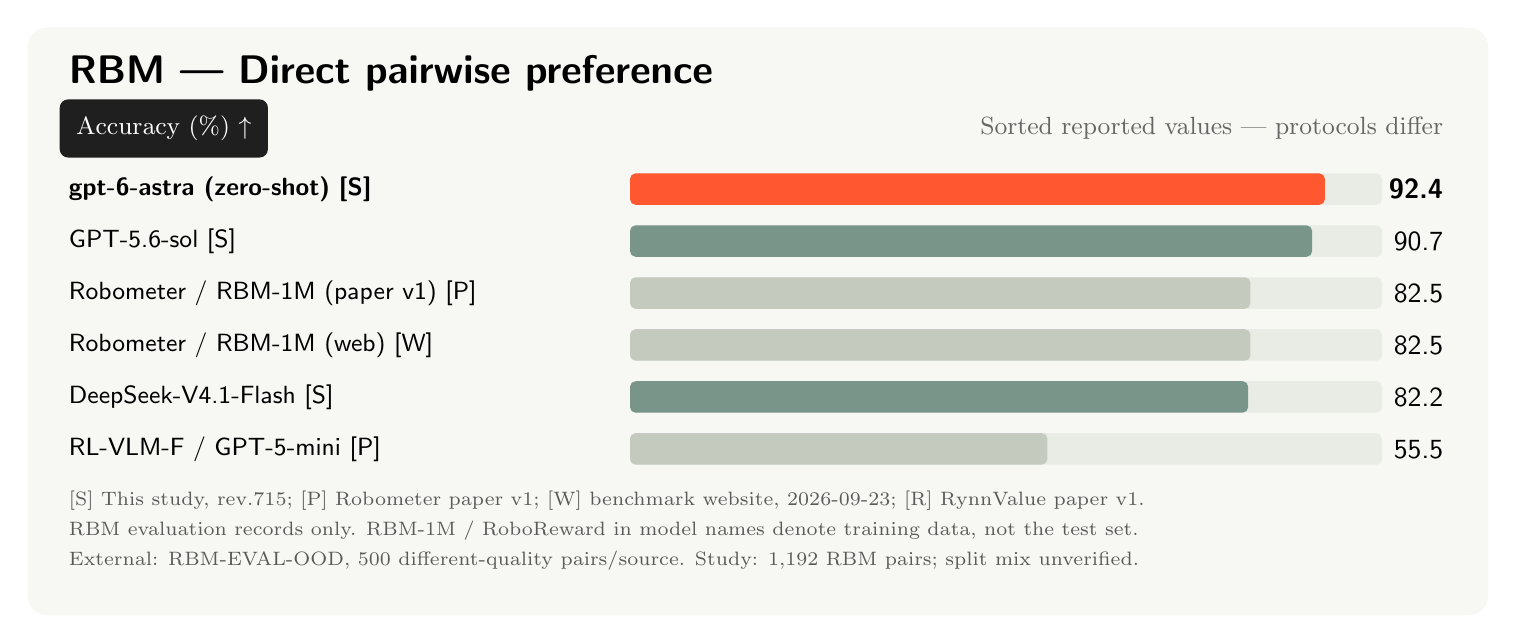
\begin{tikzpicture}[x=1cm,y=1cm,font=\sffamily]
\definecolor{cardbg}{HTML}{F7F8F3}
\definecolor{trackbg}{HTML}{E9ECE4}
\definecolor{mutedbar}{HTML}{C5CABF}
\definecolor{astrabar}{HTML}{FF572F}
\definecolor{iclbar}{HTML}{F4A082}
\definecolor{studybar}{HTML}{79958A}
\fill[cardbg,rounded corners=7pt] (-.4,1.8) rectangle (18.15,-5.66);
\node[anchor=west,font=\sffamily\bfseries\Large] at (0,1.22) {RBM | Direct pairwise preference};
\node[anchor=west,fill=black!88,text=white,rounded corners=3pt,inner sep=6pt,font=\small] at (0,.52) {Accuracy (\%) $\uparrow$};
\node[anchor=east,text=black!60,font=\small] at (17.7,.52) {Sorted reported values | protocols differ};
\node[anchor=west,font=\sffamily\small\bfseries] at (0,-0.25) {gpt-6-astra (zero-shot) [S]};
\fill[trackbg,rounded corners=2pt] (7.25,-0.45) rectangle (16.8,-0.05);
\fill[astrabar,rounded corners=2pt] (7.25,-0.45) rectangle (16.074200,-0.05);
\node[anchor=east,font=\sffamily\bfseries] at (17.7,-0.25) {92.4};
\node[anchor=west,font=\sffamily\small] at (0,-0.91) {GPT-5.6-sol [S]};
\fill[trackbg,rounded corners=2pt] (7.25,-1.11) rectangle (16.8,-0.71);
\fill[studybar,rounded corners=2pt] (7.25,-1.11) rectangle (15.911850,-0.71);
\node[anchor=east,font=\sffamily] at (17.7,-0.91) {90.7};
\node[anchor=west,font=\sffamily\small] at (0,-1.57) {Robometer / RBM-1M (paper v1) [P]};
\fill[trackbg,rounded corners=2pt] (7.25,-1.77) rectangle (16.8,-1.37);
\fill[mutedbar,rounded corners=2pt] (7.25,-1.77) rectangle (15.128750,-1.37);
\node[anchor=east,font=\sffamily] at (17.7,-1.57) {82.5};
\node[anchor=west,font=\sffamily\small] at (0,-2.23) {Robometer / RBM-1M (web) [W]};
\fill[trackbg,rounded corners=2pt] (7.25,-2.43) rectangle (16.8,-2.03);
\fill[mutedbar,rounded corners=2pt] (7.25,-2.43) rectangle (15.128750,-2.03);
\node[anchor=east,font=\sffamily] at (17.7,-2.23) {82.5};
\node[anchor=west,font=\sffamily\small] at (0,-2.89) {DeepSeek-V4.1-Flash [S]};
\fill[trackbg,rounded corners=2pt] (7.25,-3.09) rectangle (16.8,-2.69);
\fill[studybar,rounded corners=2pt] (7.25,-3.09) rectangle (15.100100,-2.69);
\node[anchor=east,font=\sffamily] at (17.7,-2.89) {82.2};
\node[anchor=west,font=\sffamily\small] at (0,-3.55) {RL-VLM-F / GPT-5-mini [P]};
\fill[trackbg,rounded corners=2pt] (7.25,-3.75) rectangle (16.8,-3.35);
\fill[mutedbar,rounded corners=2pt] (7.25,-3.75) rectangle (12.550250,-3.35);
\node[anchor=east,font=\sffamily] at (17.7,-3.55) {55.5};
\node[anchor=west,text=black!65,font=\scriptsize] at (0,-4.21) {[S] This study, rev.715; [P] Robometer paper v1; [W] benchmark website, 2026-09-23; [R] RynnValue paper v1.};
\node[anchor=west,text=black!65,font=\scriptsize] at (0,-4.59) {RBM evaluation records only. RBM-1M / RoboReward in model names denote training data, not the test set.};
\node[anchor=west,text=black!65,font=\scriptsize] at (0,-4.97) {External: RBM-EVAL-OOD, 500 different-quality pairs/source. Study: 1,192 RBM pairs; split mix unverified.};
\end{tikzpicture}
\end{document}
